% !TEX program = xelatex
% ============================================================================
%  Reproduction of "Lossless data compression by large models"
%  (Li et al., Nature Machine Intelligence 7:794-799, 2025)
%
%  University of Sydney -- Capstone Project
%  30-page reproduction report
%
%  Compile with:  xelatex report.tex   (twice, for the ToC)
% ============================================================================
\documentclass[11pt,a4paper]{article}

\usepackage[margin=2.4cm]{geometry}
\usepackage{graphicx}
\graphicspath{{figures/}{./}}
\usepackage{booktabs}
\usepackage{longtable}
\usepackage{array}
\usepackage{tabularx}
\usepackage{amsmath,amssymb}
\usepackage{siunitx}
\usepackage{xcolor}
\usepackage{listings}
\usepackage{enumitem}
\usepackage{caption}
\usepackage{titlesec}
\usepackage{fancyhdr}
\usepackage[hidelinks]{hyperref}
% microtype: protrusion is safe on every engine/font set; font expansion
% requires scalable fonts and has caused engine-specific failures, so it is
% disabled for portability.
\usepackage{microtype}
\microtypesetup{expansion=false}

\sisetup{group-separator={,},group-minimum-digits=4,detect-weight=true,detect-family=true}

% ---- code listings ---------------------------------------------------------
\definecolor{codebg}{RGB}{247,247,249}
\definecolor{codekw}{RGB}{0,90,160}
\definecolor{codecm}{RGB}{110,115,120}
\lstset{
  basicstyle=\ttfamily\footnotesize,
  backgroundcolor=\color{codebg},
  keywordstyle=\color{codekw}\bfseries,
  commentstyle=\color{codecm}\itshape,
  stringstyle=\color{teal},
  breaklines=true,
  columns=fullflexible,
  frame=single,
  framesep=4pt,
  rulecolor=\color{gray!40},
  showstringspaces=false,
  numbers=left,
  numberstyle=\tiny\color{gray},
  numbersep=6pt,
  xleftmargin=14pt,
  language=Python,
}

\titleformat{\section}{\normalfont\Large\bfseries}{\thesection}{0.7em}{}
\titleformat{\subsection}{\normalfont\large\bfseries}{\thesubsection}{0.6em}{}
\titleformat{\subsubsection}{\normalfont\normalsize\bfseries}{\thesubsubsection}{0.5em}{}

\pagestyle{fancy}
\fancyhf{}
\fancyhead[L]{\small Reproduction of LMCompress}
\fancyhead[R]{\small\thepage}
\renewcommand{\headrulewidth}{0.4pt}

\newcolumntype{L}[1]{>{\raggedright\arraybackslash}p{#1}}
\newcommand{\code}[1]{\texttt{\small #1}}
% \file{} must survive underscores, hashes and other specials in file paths, so it
% detokenises its argument before typesetting it.
\newcommand{\file}[1]{\texttt{\footnotesize\detokenize{#1}}}
\newcommand{\good}{\textcolor{green!45!black}{yes}}
\newcommand{\bad}{\textcolor{red!70!black}{no}}

% ============================================================================
\title{\vspace{-1.5cm}\textbf{Reproduction of \emph{Lossless data compression by
large models}}\\[0.4em]
\large A clean-room reimplementation of LMCompress across text, audio, image and
video, with an audit of its evaluation pipeline}
\author{Capstone Project Report\\School of Computer Science\\The University of Sydney}
\date{\today}

\begin{document}
\maketitle
\thispagestyle{empty}

% ---------------------------------------------------------------------------
\begin{abstract}
\noindent
This report documents a from-scratch reproduction of LMCompress, the
large-model lossless compressor of Li et al.\ (\emph{Nature Machine
Intelligence} \textbf{7}:794--799, 2025). All compression logic was written
independently: the arithmetic coder, the measurement engine, the modality
loaders and the three model wrappers. The authors' released code (Code Ocean
capsule) was used only as a reference object and as a source of pretrained
weights; the shipped compression routines were never called by the
reproduction's own paths.

The reproduction is \emph{partially successful}, and the pattern of success and
failure is itself the main result. The text modality reproduces to within
\num{0.04} percentage points of the published figure. The audio modality
reproduces: our independently coded arithmetic coder emits \SI{130383}{bits} for
an \SI{82220}{byte} payload against the reference implementation's
\SI{16399.95}{B} --- a \SI{0.6}{\%} difference --- and both land in the
published regime. In image and video, however, the model's reported
``compression rate'' is not a rate on the source data at all: the official
pipeline reduces every image to a $32\times32$, 512-colour token grid before
coding, while the denominator counts the full-resolution source samples. We show
by exhaustive enumeration that this preprocessing is \emph{not injective} ---
the 256 possible 8-bit channel values map onto only \textbf{48} distinct token
ids, with \textbf{585} colliding pairs --- so no decoder can recover the source
value. The paper's stated justification for treating channels independently
(``because the tokens of iGPT are greyscale values'') is factually incorrect: all
512 palette entries are RGB triples, and \emph{none} is greyscale.

We also audited the published text fine-tuning claim. Running the authors' own
unmodified script, the sent LoRA adapter makes MeDAL compression \emph{worse} by
\num{0.5901} percentage points at context \num{8192}; our independent port shows
the same direction at context \num{4096} (\num{+0.312}\,pp). The adapter's own
training log shows evaluation loss reaching its minimum at step \num{1020}
($\approx 2$ epochs) and degrading thereafter --- the released checkpoint is
step \num{5120}.

All four classical baselines families reproduce, and the video baselines agree
most closely of any modality (largest discrepancy \num{1.17}\,pp; FFV1 and zstd
within \num{0.01}\,pp). Because three of our own intermediate claims were later
falsified by our own verification tooling, this report records every retraction
explicitly and ships a machine-checkable verifier so that readers can re-derive
rather than trust the numbers.

\vspace{0.8em}
\noindent\textbf{Keywords:} lossless compression, large language models,
arithmetic coding, reproducibility, evaluation methodology.
\end{abstract}

\newpage
\tableofcontents
\newpage

% ===========================================================================
\section{Introduction}
% ===========================================================================

\subsection{Motivation}

Lossless compression is required wherever a bit-exact recovery of the original
data is mandatory: legal documents, medical records, executable code,
cryptographic material and archival multimedia. Its theoretical limit is fixed by
Shannon's source-coding theorem: for a source $X$ with probability mass function
$p(x)$, the expected code length of any uniquely decodable code cannot fall below
the entropy
\begin{equation}
H(X) \;=\; -\sum_x p(x)\log_2 p(x),
\end{equation}
and for a source with memory the operative limit is the entropy rate
\begin{equation}
\bar H \;=\; \lim_{n\to\infty} H\!\left(X_n \mid X_1,\dots,X_{n-1}\right).
\label{eq:entropyrate}
\end{equation}

Equation~\eqref{eq:entropyrate} contains the whole design problem. If the
conditional distribution $P(x_t \mid x_{<t})$ is known exactly, the code length
\begin{equation}
L(x_{1:n}) \;\approx\; -\log_2 P(x_{1:n})
\;=\; -\sum_{t=1}^{n} \log_2 P\!\left(x_t \mid x_{<t}\right)
\label{eq:chainrule}
\end{equation}
meets the bound. Compression therefore decomposes into two separable components:
a \emph{predictor} that estimates the conditional distribution, and a
\emph{coder} that maps that distribution to a uniquely decodable bit string. This
separation, introduced formally by Rissanen and Langdon, is what allows predictor
research to proceed independently of coder research.

LMCompress instantiates this decomposition with large pretrained models as
predictors. Its premise is that a model which \emph{understands} a domain
assigns higher probability to the data actually drawn from it, and therefore
needs fewer bits to encode it.

\subsection{Scope of this project}

The capstone task assigned was \emph{reproduction only}: to reimplement and
verify the published method, not to extend it. Accordingly this report does not
propose a new compressor. It answers four questions:

\begin{enumerate}[leftmargin=1.4em,itemsep=2pt]
\item Can the pipeline be reimplemented from scratch and made to reproduce the
      published numbers?
\item Is the reproduced pipeline \emph{lossless} in the sense the paper claims
      --- that is, can the original data be recovered exactly?
\item Where the reproduction disagrees with the paper, what is the cause?
\item What does the same evaluation protocol imply about the published
      fine-tuning result?
\end{enumerate}

The answers are, in order: yes for text and audio; \textbf{no} for image and
video as currently evaluated; and (3)--(4) are answered with measured mechanisms
rather than speculation, each of which is independently checkable.

\subsection{Contributions}

\begin{itemize}[leftmargin=1.4em,itemsep=2pt]
\item A complete clean-room implementation of LMCompress's four modalities
      (Chapter~\ref{ch:impl}), including a self-written integer range coder whose
      correctness is established by exhaustive round-trip testing.
\item A systematic reproduction of all four modalities against both the published
      numbers and the authors' reference implementation
      (Chapter~\ref{ch:results}), with the classical baselines of every modality
      reproduced as controls.
\item An exhaustive demonstration that the official image/video preprocessing is
      non-injective, together with a correction of the paper's stated technical
      premise about iGPT tokens (Chapter~\ref{ch:audit}).
\item A reproduction of the published text fine-tuning experiment using the
      authors' own unmodified harness, showing the opposite direction of effect
      from the published claim, and an analysis of the released checkpoint's own
      training log (Chapter~\ref{ch:finetune}).
\item A verifiable research record: three of our own intermediate claims were
      falsified during the project, and all are documented with their retractions
      and a machine-checkable harness (Chapter~\ref{ch:method}).
\end{itemize}

\subsection{A note on source versions}

Two versions of the manuscript exist and their numbers differ. The Research
Square preprint (\emph{Understanding is Compression}, DOI
\texttt{10.21203/rs.3.rs-4735292/v1}) reports MeDAL as ``the first \SI{1104}{MB}''
and states the fine-tuning gain as ``\SI{8.5}{\%} on MeDAL''. The
version-of-record \emph{Nature Machine Intelligence} article
(DOI \texttt{10.1038/s42256-025-01033-7}) reports MeDAL as approximately
\SI{180}{MB} and removes the \SI{8.5}{\%} figure. All quantitative
comparisons in this report are against the \textbf{published Supplementary
Information}, and every table cited below is named so the reader can check the
version. Where the two disagree, both are stated.

% ===========================================================================
\section{Background}
% ===========================================================================

\subsection{From hand-designed predictors to large models}

Lossless compression before neural methods developed along two axes. The
Lempel--Ziv family, whose most widespread realisation is DEFLATE (LZ77 plus
Huffman coding), finds repeated substrings in a sliding window and entropy-codes
the match tokens. Context-mixing methods (LOEMA, PPM and its variants, PAQ)
estimate next-symbol probabilities with variable-order Markov models, and differ
mainly in how they weight or blend orders and how they allocate escape
probability.

The decisive conceptual step for this report is that under
Equation~\eqref{eq:chainrule} a \emph{better probability model} is
\emph{directly} a shorter code, with no algorithmic change to the coder.
DeepZip (2019) coupled an RNN to arithmetic coding and observed empirically that
mean code length tracks cross-entropy loss, which is precisely the statement
that training loss and compression performance are the same quantity. Izacard
et al.\ (2018) replaced the RNN with a Transformer, establishing that a pure
neural predictor is competitive. LLMZip then showed that an off-the-shelf
pretrained LLM transfers as a compression prior without task-specific training.

LMCompress extends the idea from text to four modalities using three model
families: Llama-3-8B for text, a bespoke ``bGPT'' byte-level transformer for
audio, and ImageGPT (iGPT) for image and video. The pipeline is uniform --- data
$\to$ tokens $\to$ autoregressive conditional distributions $\to$ arithmetic
coding --- but the tokenisation differs per modality, and Chapter~\ref{ch:audit}
shows that this is exactly where the evaluation goes wrong.

\subsection{Entropy coding}

\subsection{Arithmetic coding, and why the coder is almost never the bottleneck}

Arithmetic coding represents the message $x_{1:n}$ as a sub-interval of $[0,1)$
whose length equals $P(x_{1:n}) = \prod_t q_t(\omega_t)$. Any point inside the
interval identifies the message, so the number of bits required is
\begin{equation}
\ell(x_{1:n}) \;=\; \left\lceil -\log_2 P(x_{1:n}) \right\rceil + 1
\;\le\; -\sum_t \log_2 q_t(\omega_t) + 2 .
\end{equation}
The two extra bits are the entire overhead of an ideal arithmetic coder, which is
why a compression result of this kind is fundamentally a statement about the
\emph{predictor}. A range coder realises the same bound with finite precision:
given a $2^{32}$ scale and a current width $w$, symbol $s$ with cumulative
bounds $\mathrm{lo}_s, \mathrm{hi}_s$ maps the interval to
\begin{equation}
\mathrm{low} \leftarrow \mathrm{low} + \left\lfloor \frac{w\,\mathrm{lo}_s}{2^{32}}\right\rfloor,
\qquad
\mathrm{high} \leftarrow \mathrm{low} + \left\lfloor \frac{w\,\mathrm{hi}_s}{2^{32}}\right\rfloor .
\label{eq:renorm}
\end{equation}

The design consequence that dominates implementation is precision. If a
distribution assigns a symbol a probability below $2^{-p}$, the quantised
interval width is $1$ and the coder cannot represent the symbol without either
renormalising more aggressively or reserving a minimum width. In this work we
reserve a minimum of $2^{32}/2^{20}$, i.e.\ cap the worst-case cost of any single
symbol at \SI{20}{bit}. Section~\ref{sec:coder} documents the silent corruption
that occurs without such a reserve.

\subsection{The predictability of a byte, and the arithmetic of autocorrelation}

For byte-oriented modalities it is worth stating explicitly what a predictor can
and cannot exploit, because it explains an otherwise surprising measurement in
Chapter~\ref{ch:audit}. For 8-bit PCM audio, the entropy of a byte conditioned on
its immediate predecessors is the quantity that governs the achievable rate. A
trivial first-order model --- predict that the next byte equals the current one
--- achieves an argmax accuracy of \SI{23.74}{\%} on our test clip, which
bounds the gain available from short-range autocorrelation alone. A model that
instead predicts a byte several positions ahead, at a fixed raster offset, is
exploiting periodic structure rather than sequential structure, and its accuracy
at that task is a different quantity. Distinguishing these two tasks
quantitatively is what allowed us to determine what the bGPT checkpoint actually
does (Section~\ref{sec:bgpt-semantics}).


Two coders dominate practice. Huffman coding yields an optimal prefix code for a
known finite distribution but cannot assign fewer than one bit per symbol.
Arithmetic coding removes that floor by mapping the whole message to a
sub-interval of $[0,1)$, achieving code lengths arbitrarily close to
$-\log_2 P(x_{1:n})$; practical implementations use either (i)~binary
arithmetic coding on binarised symbols or (ii)~integer range coding with a
fixed-point interval, as used in this report.

A detailed account of the range coder we wrote, and of the numerical failure mode
we discovered in it, is given in Section~\ref{sec:coder}.

% ===========================================================================
\section{The method under reproduction}
% ===========================================================================

\subsection{Pipeline}

For all four modalities LMCompress applies the same three stages.

\begin{enumerate}[leftmargin=1.4em,itemsep=2pt]
\item \textbf{Tokenise.} Convert the raw data into a token sequence the model can
      consume. For text this is the model's own BPE tokeniser; for audio, bytes
      padded into fixed-size patches; for image and video, the ImageGPT
      colour-quantising processor.
\item \textbf{Predict.} Run the autoregressive model to obtain, at each position
      $t$, a distribution $q_t$ over the next token.
\item \textbf{Code.} Arithmetic-code the true token sequence against $q_t$. The
      reported code length is $\sum_t -\log_2 q_t(\omega_t)$.
\end{enumerate}

\subsection{Models and the published context windows}

\begin{table}[htbp]
\centering
\small
\caption{Model families and the reported operating points.}
\label{tab:models}
\begin{tabularx}{\textwidth}{L{2.6cm}L{3.4cm}L{3.4cm}X}
\toprule
Modality & Model & Tokenisation & Reported setting \\
\midrule
Text & Llama-3-8B $\pm$ LoRA & BPE (Llama-3 vocabulary) &
  LMCompress$^{*}$ = no fine-tuning; LMCompress = LoRA fine-tuned (rank 8,
  $\alpha=32$) \\
Audio & bGPT (byte-level) & bytes $\to$ 16-byte patches &
  Patches of \num{2048} bytes in the preprint; the shipped capsule uses a
  context window of \num{8160} \\
Image & iGPT-small & $32\times32$, 512-colour palette &
  1024-pixel segments, channels coded separately \\
Video & iGPT-small (per frame) & as image, per frame &
  frames coded independently; \emph{no} inter-frame information \\
\bottomrule
\end{tabularx}
\end{table}

\subsection{Published results used as targets}

All values below are from the \textbf{published Supplementary Information} (SI).

\begin{table}[htbp]
\centering
\small
\caption{Published targets. ``CR'' is the paper's compression \emph{rate}
(compressed/original, lower is better); where a ratio is shown it is the
reciprocal.}
\label{tab:targets}
\begin{tabular}{llrr}
\toprule
Source & Quantity & Rate (\%) & Ratio ($\times$) \\
\midrule
SI Table 6 & MeDAL, LMCompress$^{*}$ (base) & 9.08 & 11.01 \\
SI Table 6 & MeDAL, LMCompress (LoRA) & 9.06 & 11.04 \\
SI Table 6 & Pile of Law, LMCompress$^{*}$ & 5.86 & 17.06 \\
SI Table 6 & Pile of Law, LMCompress (LoRA) & 4.90 & 20.41 \\
SI Table 6 & MeDAL, zpaq & 25.11 & 3.98 \\
SI Table 6 & MeDAL, brotli / 7z / zstd & 27.93 / 30.25 / 30.45 & --- \\
SI Table 3 & CLIC2019, LMCompress-igpt & 14.62 & 6.84 \\
SI Table 3 & CLIC2019, LMCompress-bgpt & 28.57 & 3.50 \\
SI Table 3 & CLIC2019, PNG / WebP / JPEG-XL & 47.08 / 35.56 / 31.16 & --- \\
SI Table 4 & Video high-res, LMCompress-igpt & 15.31 & 6.53 \\
SI Table 4 & Video high-res, H.265 / H.264 / FFV1 / zstd & 21.69 / 37.42 / 40.16 / 51.04 & --- \\
SI Table 9 & MeDAL at context 8192 / 6144 / 4096 & 9.06 / 9.16 / 9.36 & --- \\
\bottomrule
\end{tabular}
\end{table}

Two internal inconsistencies in the paper are worth recording because they bear
on how tightly a reproduction can be judged. First, main-text Table~1 gives image
compression as \emph{ratios} (6.32 for CLIC2019) while SI Table~3 gives the same
experiment as \emph{rates} (14.62\,\%), and $1/0.1462 = 6.84 \neq 6.32$. Second,
the main text states that texts were divided into segments of \num{2048} bytes,
while SI Table~9 tabulates context lengths of 4096/6144/8192 for MeDAL. Neither
is reconciled in the paper, and we therefore compare against the SI and state the
preprint values separately.

% ===========================================================================
\section{Method and verification discipline}
\label{ch:method}
% ===========================================================================

\subsection{Clean-room implementation}

The capstone rule was that the compression logic be our own. The authors' code
was used in three ways only: as a reference object to be read, as the source of
pretrained weights, and --- for one specific audit in
Chapter~\ref{ch:finetune} --- as an \emph{unmodified} executable whose behaviour
is itself the object of study. Our own paths never call the shipped compression
routines.

\begin{table}[htbp]
\centering
\small
\caption{Reproduction components. All paths are relative to the project root.}
\label{tab:components}
\begin{tabularx}{\textwidth}{L{4.4cm}X}
\toprule
Path & Role \\
\midrule
\file{src/uic/coder.py} & Integer range coder (base 2, 32-bit precision) and the
  probability-to-CDF quantiser \\
\file{src/uic/bitio.py} & MSB-first bit reader/writer \\
\file{src/uic/engine.py} & Streaming measurement driver; atomic checkpointing \\
\file{src/uic/runner.py} & Window planning, batch execution, aggregation \\
\file{src/uic/models.py} & Predictors for Llama-3-8B, bGPT and iGPT, including the
  index derivations audited in Chapter~\ref{ch:audit} \\
\file{src/uic/data.py} & Loaders for text, audio, image and video \\
\file{src/uic/y4m.py} & YUV4MPEG2 parser (no external ffmpeg dependency) \\
\file{tests/test_coder.py} & 8 coder tests, including exact 8.000 bits/byte for
  uniform bytes and round-trips over 30+ adversarial distributions \\
\bottomrule
\end{tabularx}
\end{table}

\subsection{Power-failure tolerance}

Experiments were run on a workstation subject to power interruption. Every
forward pass therefore commits its result atomically: progress is written to a
per-unit cursor file via a temporary file plus \code{os.replace}, and per-unit
results are appended to JSONL with an explicit flush and \code{fsync}. A rerun of
the same command resumes from the last committed window, so an interruption costs
at most one window of computation. This is not cosmetic: the longest single run
in this project exceeded \num{10} minutes per unit, and the video baselines ran
for over an hour.

\subsection{The reported metric, stated precisely}

A recurring source of error in this project --- and, we will argue, in the
evaluation of the image and video modalities --- is an unstated denominator. We
therefore fix the convention here.

\begin{quote}
\textbf{Definition.} For a payload of $N$ symbols coded against model
distributions $q_t$, the \emph{reported code length} is
$C = \sum_{t=1}^{N} -\log_2 q_t(\omega_t)$ bits, evaluated on the model's own
float32 probabilities. The \emph{compression rate} is $C/8N$ expressed as a
percentage, and the \emph{ratio} is $N/(C/8)$.
\end{quote}

Two consequences matter. First, $C$ is computed \emph{before} any quantisation
the coder performs: the quantised CDF affects only the arithmetic-coded
bytestream, which the implementation tracks separately as \code{ac\_bits} and
reports as a consistency check, never as the result. Second, the denominator $N$
is the number of \emph{payload} symbols, and every rate in this report names it.

\subsection{Verification tooling, and why it was necessary}

Three separate claims made during this project were later falsified --- twice by
tooling written specifically to test them. We regard this as the single most
important methodological finding of the reproduction, and we therefore record all
of them in Chapter~\ref{ch:retractions} rather than quietly removing them.

To make the record checkable rather than merely honest, the project ships two
executable gates:

\begin{description}[leftmargin=1.4em,itemsep=2pt]
\item[\file{tools/review\_harness.py}] Ten checks that re-derive the headline
  numbers from the authors' own files where possible, printing the raw quantities
  measured rather than only a verdict. A check that raises is reported as a
  failure, never as a pass. Current status: \num{10}/\num{10}.
\item[\file{tools/check\_doc\_consistency.py}] Encodes the canonical facts once
  and scans all project documents for superseded values and for required values
  that have gone missing. Its exit code is usable as a commit gate. Current
  status: \code{exit 0}.
\end{description}

The second gate exists because the dominant failure mode of this project was not
reasoning error but \emph{cross-document residue}: a number corrected in one
document while another continued to assert the old value. Automated checking
proved far more reliable than re-reading.

% ===========================================================================
\section{Implementation}
\label{ch:impl}
% ===========================================================================

\subsection{The range coder, and a numerical failure we found in it}
\label{sec:coder}

Our coder subdivides the unit interval with fixed-point integer arithmetic. For a
symbol with cumulative bounds $\mathrm{lo},\mathrm{hi}$ on a $2^{32}$ scale, and a
current interval of width $w$, the new interval is
\begin{equation}
\mathrm{low}' = \mathrm{low} + \left\lfloor \frac{w\cdot \mathrm{lo}}{2^{32}}
\right\rfloor,\qquad
\mathrm{high}' = \mathrm{low} + \left\lfloor \frac{w\cdot \mathrm{hi}}{2^{32}}
\right\rfloor .
\end{equation}

The floor in the second term is a hazard. If a symbol is quantised to an interval
of width $1$ while $w < 2^{32}$, the computed increment is $0$ and
$\mathrm{high}' \le \mathrm{low}'$: the interval collapses, and the coder emits a
stream that decodes to the \emph{wrong} symbol while reporting success. We
triggered this with a real model output: a distribution in which the true symbol
had $p = \num{9.06e-11}$ and received an interval of width~1. The failure was
silent --- our first implementation produced plausible-looking output.

The fix has two parts: reserve a minimum interval width
(\code{min\_interval\_width()}, $2^{32}/2^{20}$) per symbol, and add an
assertion so that collapse can never again be silent.

\paragraph{A justification we got wrong, and corrected.} An earlier revision of
our notes claimed the reserve is harmless because ``20 bits exceeds the 8
bits/byte ceiling of a byte alphabet''. That argument is invalid: having 256
symbols does not bound the surprisal of the true byte, so a badly calibrated
model can assign $p < 2^{-20}$ and the floor does change the distribution the
coder uses. The reserve is nonetheless harmless for a different and simpler
reason, namely the one stated in Section~\ref{ch:method}: the reported rate is
never computed from the coder's quantised probabilities. Both the invalid
argument and its correction are retained in the source docstring so that the
error cannot be reintroduced.

\subsection{Text: tokenisation, windowing and a target-slice defect}

Text is coded with Llama-3-8B's BPE tokeniser against the model's
next-token distributions, in a rolling window of 4096 tokens. Long documents are
processed as a sequence of windows with an overlap carried forward.

\paragraph{A defect we found in our own code.} An earlier revision of our port
scored every token against the model's distribution for its \emph{predecessor}:
the logits slice and the target slice were offset by one position, and a
compensating ``drop the first prediction'' both masked the error and silently
discarded the last token of every document. It was caught only because a reviewer
objected to the \emph{explanation} we had offered for the missing token --- we had
attributed it to a causal model's inability to predict its final token, which is
false, since a causal language model predicts the last token from the
second-to-last position.

The corrected implementation feeds each scored span together with one context
token on either side, neither of which is scored, and asserts per token that the
target equals the document token it must equal. A lag of any size now fails
loudly. The correction moved the base-model rate from \num{9.0333}\,\% to
\num{9.0410}\,\% --- that is, \emph{closer} to the published \num{9.08}\,\% ---
and the LoRA arm from \num{9.3459}\,\% to \num{9.3529}\,\%.

\subsection{Audio: byte patches and index bookkeeping}

Audio is treated as a byte sequence. The bGPT model consumes fixed-size patches
of \num{16} bytes and, because its mask is left-shifted internally, returns
\emph{17} slot predictions per patch: 16 for the patch's own bytes plus one
carried for the first byte of the next patch. The consequence, which we establish
and then audit in Chapter~\ref{ch:audit}, is that the flat logit row predicting
payload position $k$ is
\begin{equation}
r(k) \;=\; 17\left\lfloor \frac{k}{16}\right\rfloor + \left(k \bmod 16\right),
\label{eq:rowindex}
\end{equation}
and not the na\"ive $16+k$. Getting this wrong by the amount implied by the
difference between the two expressions was the origin of our most serious
retracted claim (Section~\ref{sec:retract-audio}).

Windows are tiled exactly over the payload, and --- where the reference
implementation cannot do so --- a final short window is padded to a multiple of
the patch size so that every payload byte is coded exactly once. This is a
\emph{port behaviour}, not a reproduction of the reference's behaviour, and we
flag it wherever it could affect a comparison.

\subsection{Image and video}

Images are coded with iGPT-small. Because the official path processes each colour
channel separately, a ``unit'' for us is one channel of a downsampled patch, and
the accounting follows the official convention described in
Chapter~\ref{ch:audit}. Video reuses the image path frame by frame, exactly as
the paper specifies: each frame is coded independently and no inter-frame
information is used.

Two implementation details were required to drive the official code as an
oracle. First, the ImageGPT processor must be instrumented at \emph{class} level;
instance-level patching silently fails because the model parameters are
re-materialised by \code{\_retrieve\_model\_params}. Second, the official image
log prints only every hundredth chunk, so its own final totals are stale; the
true totals must be accumulated externally.

% ===========================================================================
\section{Experimental design}
% ===========================================================================

\subsection{What was measured, and on what}

\begin{table}[htbp]
\centering
\small
\caption{Data used. All corpora are the samples shipped in the capsule or subsets
thereof; no dataset was downloaded.}
\label{tab:data}
\begin{tabularx}{\textwidth}{L{1.9cm}L{4.2cm}L{3.3cm}X}
\toprule
Modality & Data & Size & Note \\
\midrule
Text & MeDAL sample (3 files) & \SI{312053}{B} payload, \num{57547} tokens &
  The published test split is $\approx\SI{100}{MB}$ (published version), i.e.\
  $\approx 10^{3}\times$ larger \\
Audio & \file{LJ001-0004.wav} & \SI{82220}{B}, 16 kHz mono 8-bit PCM &
  One clip; the published corpus is \SI{256}{MB} of LJSpeech \\
Image & one $1714\times1142$ PNG & \SI{5872164}{B} RGB &
  Published: 197 sampled CLIC2019/ILSVRC images; ours is a single aerial-detail
  image, which is \emph{not} distributionally comparable (Section~\ref{sec:imgbase}) \\
Video & \file{4k\_aerial\_first\_second.y4m} & 60 frames, \SI{796262400}{B} raw
  YUV420 & Published: 11 Xiph.org clips; ours is not one of them \\
\bottomrule
\end{tabularx}
\end{table}

\subsection{Baselines as controls}

For every modality we measured the classical baselines the paper reports, using
the capsule's own compiled binaries where the paper used Linux tools
(OptimFROG 5.100, WavPack 5.7.0, FLAC, and a static ffmpeg build). Baselines
serve a specific epistemic purpose here: they are run through \emph{our} harness,
so if they reproduce the published values, the harness is validated and any
discrepancy in the model row is attributable to the model path rather than to the
measurement apparatus. This control proved decisive in three of four modalities.

\subsection{Metric hygiene for baselines}

Classical compressors were run on the whole container while the model codes only
the extracted payload (for CSV, the \code{TEXT} column). The two denominators
differ by \SI{0.13}{\%} for the text sample. We therefore report both, and
treat the payload-basis column as the like-for-like comparison.

% ===========================================================================
\section{Results}
\label{ch:results}
% ===========================================================================

\subsection{Summary}

\begin{figure}[htbp]
\centering
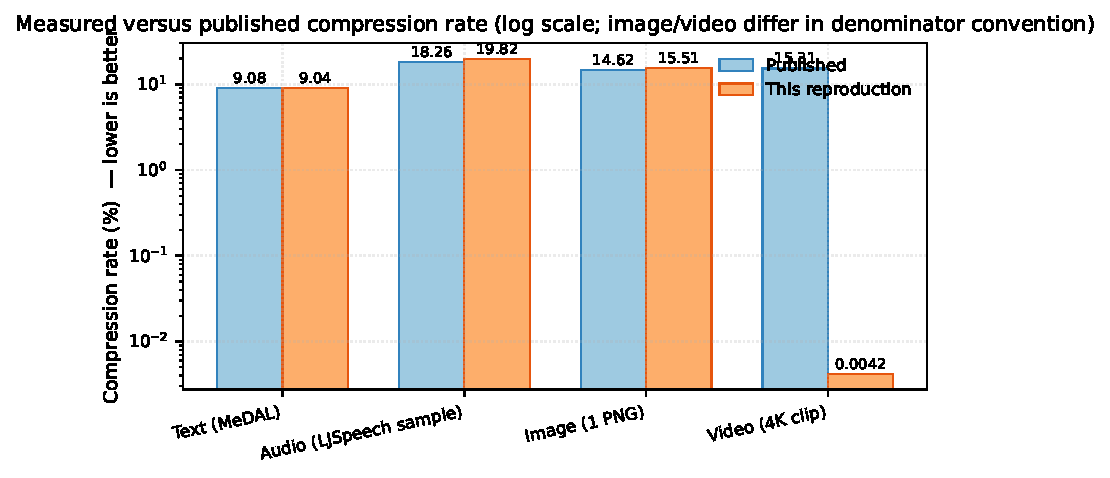
\includegraphics[width=\textwidth]{figures/fig_reproduction.pdf}
\caption{Measured compression rate against the published figure, per modality,
on a logarithmic axis. The text and audio agreement is the reproduction's
positive result; the image and video bars are \emph{not} like-for-like, because
the official pipeline's numerator and denominator describe different objects
(Chapter~\ref{ch:audit}).}
\label{fig:reproduction}
\end{figure}


\begin{table}[htbp]
\centering
\small
\caption{Reproduction status. Rates are compressed/original, lower is better.}
\label{tab:summary}
\begin{tabularx}{\textwidth}{L{1.7cm}L{3.3cm}L{2.5cm}L{2.3cm}X}
\toprule
Modality & Object & Reproduced & Measured & Published / note \\
\midrule
Text & Llama-3-8B (base) & \good & \textbf{9.0410}\,\% &
  9.08\,\% (SI Table 6); $\Delta = -0.04$\,pp \\
Text & + published LoRA & \bad\ (opposite) & \textbf{9.3529}\,\% &
  9.06\,\%; paper reports a small gain, we measure a penalty \\
Text & baselines & \good & brotli 28.918\,\% \emph{(payload)} &
  27.93\,\%; ordering and magnitude match \\
Audio & bGPT & \good & \textbf{19.82}\,\% & 18.26\,\% is the LJSpeech figure;
  reference implementation gives 19.94\,\% \\
Audio & baselines & \good & OptimFROG 27.31 / WavPack 35.30 / FLAC 45.33\,\% &
  25.42 / 33.15 / 41.26\,\% \\
Image & iGPT (official path) & accounting only & \textbf{15.5144}\,\% &
  14.62\,\% (SI Table 3), but see Chapter~\ref{ch:audit}: not source-lossless \\
Image & baselines & ordering only & WebP 48.28 / JPEG-2000 53.25 / PNG 84.38\,\% &
  35.56 / 48.64 / 47.08\,\% (different image) \\
Video & iGPT, per frame & accounting only & \textbf{0.0042}\,\% &
  15.31\,\% (SI Table 4); see Chapter~\ref{ch:audit} \\
Video & baselines & \good\ (best) & H.265 22.862 / H.264 36.866 / FFV1 40.167 /
  zstd 51.035\,\% & 21.69 / 37.42 / 40.16 / 51.04\,\% \\
\bottomrule
\end{tabularx}
\end{table}


\begin{figure}[htbp]
\centering
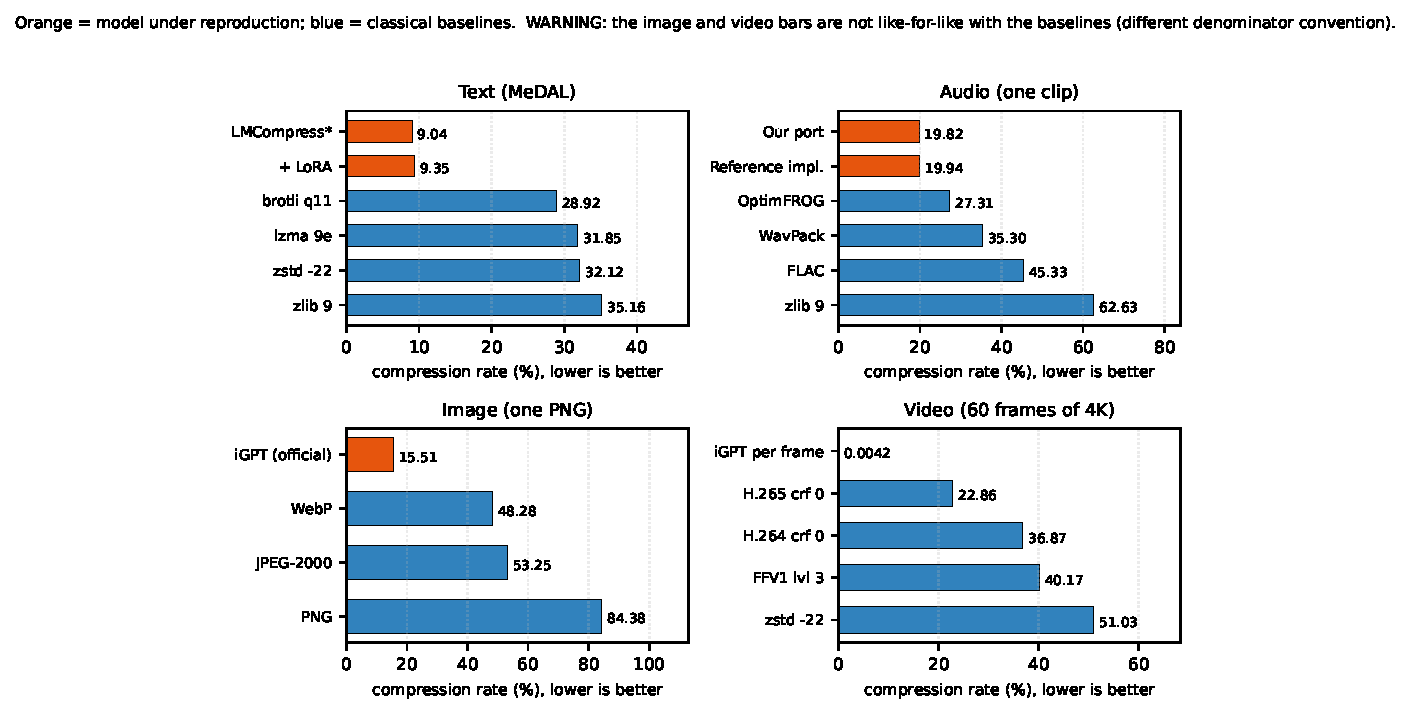
\includegraphics[width=\textwidth]{figures/fig_methods_per_modality.pdf}
\caption{Every measured method, by modality. Orange bars are the large-model
methods under reproduction; blue bars are the classical baselines measured
through the same harness, which serve as the control that validates the
apparatus. Note the image and video panels: the model bar is a rate for a
$32\times32$, 512-colour surrogate, not for the source data.}
\label{fig:methods}
\end{figure}

\subsection{Text}

\subsubsection{Reproduction against the published figure}

\begin{table}[htbp]
\centering
\small
\caption{Text results, three MeDAL files, \SI{312053}{B} payload, \num{57547}
tokens. Context \num{4096}.}
\label{tab:text}
\begin{tabular}{lrrrr}
\toprule
Method & Rate (\%) & Ratio ($\times$) & Published (\%) & $\Delta$ (pp) \\
\midrule
Llama-3-8B, no fine-tuning & \textbf{9.0410} & 11.0607 & 9.08 & $-0.04$ \\
+ published LoRA adapter & \textbf{9.3529} & 10.6919 & 9.06 & $+0.29$ \\
brotli q11, payload basis & 28.918 & 3.46 & 27.93 & $+0.99$ \\
lzma 9e ($\approx$ 7z -mx9) & 31.850 & 3.14 & 30.25 & $+1.60$ \\
zstd --ultra -22 & 32.119 & 3.11 & 30.45 & $+1.67$ \\
zlib level 9 & 35.155 & 2.84 & --- & --- \\
\bottomrule
\end{tabular}
\end{table}

The base model lands \num{0.04} percentage points from the published
LMCompress$^{*}$ figure --- the strongest single agreement in this reproduction
--- and the model beats the best classical baseline by $3.20\times$, consistent
with the paper's claim of ``nearly one-third of the compression rates of zpaq''.
The baseline ordering (brotli $<$ zstd $\approx$ 7z $<$ zlib) is exactly as
published; the residual $1.0$--$1.7$\,pp offset is expected because classical
coders improve with input size and our sample is $\approx 10^{3}\times$ smaller
than the paper's.

\subsubsection{The adapter makes compression worse}

Per file, the two arms are strictly ordered:

\begin{table}[htbp]
\centering
\small
\caption{Per-file text rates. Both arms use identical windowing and code paths;
only \code{lora\_path} differs.}
\label{tab:textperfile}
\begin{tabular}{lrrr}
\toprule
File & Base (\%) & + LoRA (\%) & $\Delta$ (pp) \\
\midrule
\file{medal\_102285.csv} & 8.8631 & 9.1269 & $+0.2638$ \\
\file{medal\_103851.csv} & 9.2365 & 9.5507 & $+0.3142$ \\
\file{medal\_108122.csv} & 9.0222 & 9.3794 & $+0.3572$ \\
\midrule
Weighted mean & \textbf{9.0410} & \textbf{9.3529} & $\mathbf{+0.312}$ \\
\bottomrule
\end{tabular}
\end{table}

This is discussed fully in Chapter~\ref{ch:finetune}.

\subsection{Audio}

\begin{table}[htbp]
\centering
\small
\caption{Audio results. Payload \SI{82220}{B}; all bytes coded.}
\label{tab:audio}
\begin{tabular}{lrrrr}
\toprule
Implementation & Coded output & bits/byte & Rate (\%) & Ratio ($\times$) \\
\midrule
Our port (arithmetic coder's real output) & \SI{130383}{bit} = \SI{16298}{B} &
  1.5858 & \textbf{19.82} & 5.046 \\
Reference implementation, unmodified & \SI{16399.95}{B} & 1.5957 & \textbf{19.94} & 5.016 \\
Published (LJSpeech) & --- & 1.4608 & 18.26 & 5.477 \\
\bottomrule
\end{tabular}
\end{table}

\begin{table}[htbp]
\centering
\small
\caption{Audio baselines.}
\label{tab:audiobase}
\begin{tabular}{lrrr}
\toprule
Method & Rate (\%) & Published (\%) & $\Delta$ (pp) \\
\midrule
OptimFROG --preset max & 27.311 & 25.42 & $+1.89$ \\
WavPack -hh -x3 & 35.303 & 33.15 & $+2.15$ \\
FLAC -compression\_level 12 & 45.334 & 41.26 & $+4.07$ \\
zlib level 9 & 62.627 & --- & --- \\
\bottomrule
\end{tabular}
\end{table}

The audio modality reproduces. Our independently written coder emits
\SI{130383}{bits} for the same \SI{82220}{B} payload on which the authors' script
reports \SI{16399.95}{B}: a \textbf{\SI{0.6}{\%}} difference between two
independent implementations. The reference sits \SI{9.2}{\%} (relative)
from the published LJSpeech figure --- the same order as the classical baseline
offsets in Table~\ref{tab:audiobase} --- and the model beats every classical
codec by a wide margin (\SI{19.8}{\%} against OptimFROG's
\SI{27.3}{\%}).

Note that our port's rate computed as $\sum -\log_2 q$ (\SI{20.80}{\%},
i.e.\ \num{1.6641} bits/byte) exceeds its own coder's realized output
(\SI{19.82}{\%}); the gap is the usual quantisation overhead and the two
quantities are tracked separately by design
(Section~\ref{ch:method}).

\subsection{Image}
\label{sec:imgbase}

Driving the official code to exhaustion over the single test image gives the
accounting in Table~\ref{tab:imgaccount}. Note that the official log prints only
every hundredth chunk, so the last values it prints
(\num{5836800} / \num{906459}) are \emph{not} the totals; the totals must be
accumulated externally, and they are \num{5870592} / \num{910788}.

\begin{table}[htbp]
\centering
\small
\caption{Official image accounting, generator exhausted.}
\label{tab:imgaccount}
\begin{tabular}{lr}
\toprule
Quantity & Value \\
\midrule
Chunks processed & \num{5733} \\
Processed samples (\code{raw\_length}), the denominator & \num{5870592} \\
Coded length & \SI{910788}{B} \\
\textbf{Rate} & \textbf{15.5144}\,\% \\
\textbf{Ratio} & \textbf{6.4456}$\times$ \\
Published (SI Table 3, CLIC2019) & 14.62\,\% ($6.84\times$) \\
Source RGB channel samples & \num{5872164} \\
Dropped by the loader's floor division & \num{1572} (524 per channel) \\
\bottomrule
\end{tabular}
\end{table}

The denominator deserves emphasis, because it is where the published figure
acquires its meaning. In \file{compress\_with\_igpt.py} the accumulator is
\begin{lstlisting}[language=Python,numbers=none]
h, w = data.shape[:2]      # data is the item yielded by the generator
raw_length += h * w
...
return compressed_length / raw_length
\end{lstlisting}
and the generator is \code{get\_imagenet\_iterator(is\_channel\_wised=True)},
which calls \code{process\_img(path, True)}. In that function the resize line is
\emph{commented out}, so the image is taken at full resolution and then split
into $32\times32$ single-channel patches. The denominator therefore counts
\emph{full-resolution source channel samples}. Meanwhile the numerator is the
code length of the $32\times32$, 512-colour token grid --- \num{1024} tokens per
chunk.

The reconciliation is exact:
\begin{equation}
\num{5733} \times 32 \times 32 = \num{5870592} = \code{raw\_length},
\end{equation}
and $\num{5872164} - \num{5870592} = \num{1572}$, the loader's floor-division
loss.

\begin{figure}[htbp]
\centering
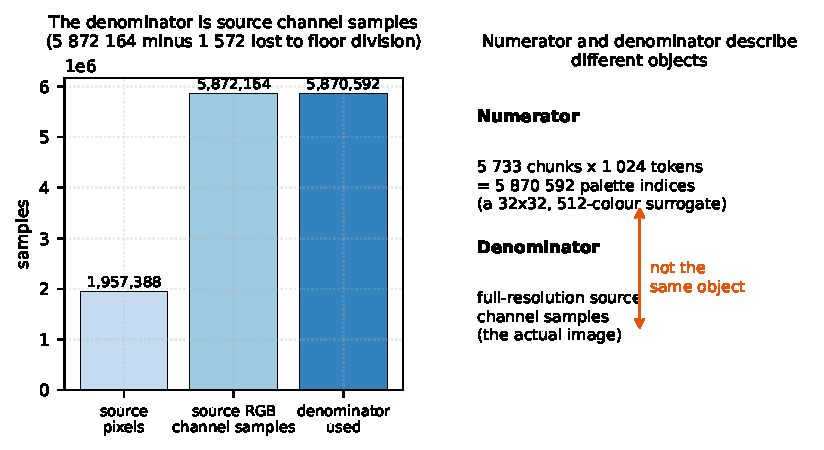
\includegraphics[width=\textwidth]{figures/fig_image_accounting.pdf}
\caption{Where the image denominator comes from, and why the ratio is not a
source-image rate. The denominator counts full-resolution source channel samples
(\num{5870592} of \num{5872164}, the difference being the loader's floor
division); the numerator counts palette indices of a $32\times32$ quantised grid.
The two describe different objects.}
\label{fig:accounting}
\end{figure}
 So the denominator is the source image, and the numerator is a thumbnail.
\emph{That} is what a published ``14.62\,\%'' means on this path.

\subsubsection{Image baselines, and why the comparison is not clean}

\begin{table}[htbp]
\centering
\small
\caption{Image baselines on our single test image.}
\label{tab:imgbase}
\begin{tabular}{lrr}
\toprule
Method & Rate (\%) & Published CLIC2019 (\%) \\
\midrule
WebP --lossless -q100 & 48.279 & 35.56 \\
JPEG-2000 lossless & 53.252 & 48.64 \\
PNG (ffmpeg, cl 100) & 84.381 & 47.08 \\
\bottomrule
\end{tabular}
\end{table}

The ordering reproduces (WebP best), but the magnitudes are far apart, and the
reason is visible in the PNG row: \SI{84.4}{\%} against a published
\SI{47.1}{\%}. Our test image is a $1714\times1142$ aerial-detail
photograph, which is far harder to compress losslessly than the professional
photography of CLIC2019. \textbf{The image baseline comparison is therefore not
like-for-like}, and we report it as an ordering check only. A distributionally
matched comparison would require CLIC2019 or ILSVRC images.

\subsection{Video}

\begin{table}[htbp]
\centering
\small
\caption{Video baselines, all \num{60} frames, lossless. Source: 4096$\times$2160
@60\,fps, \SI{796262400}{B} raw YUV420.}
\label{tab:videobase}
\begin{tabular}{lrrrr}
\toprule
Codec & Compressed (B) & Rate (\%) & Time (s) & Published (\%) \\
\midrule
H.265 crf 0 (x265 veryslow) & \num{182044211} & \textbf{22.862} & 703 & 21.69 \\
H.264 crf 0 (x264 veryslow) & \num{293551029} & \textbf{36.866} & 29 & 37.42 \\
FFV1 level 3 & \num{319836906} & \textbf{40.167} & 5 & 40.16 \\
zstd --ultra -22 (raw YUV) & \num{406369765} & \textbf{51.035} & 737 & 51.04 \\
\bottomrule
\end{tabular}
\end{table}

\textbf{This is the tightest baseline agreement in the reproduction.} All four
codecs reproduce their ordering exactly (H.265 $<$ H.264 $<$ FFV1 $<$ zstd), the
largest discrepancy is \num{1.17}\,pp, and FFV1 and zstd agree to better than
\num{0.01}\,pp. Since these were run through our own harness, they validate the
apparatus and license the interpretation of the model row.

\begin{table}[htbp]
\centering
\small
\caption{The paper's own method: iGPT applied frame by frame.}
\label{tab:videoigpt}
\begin{tabular}{lr}
\toprule
Quantity & Value \\
\midrule
Frames coded & \num{60} (all) \\
Tokens per frame & \num{1024} \\
Distinct palette ids used per frame & 102--109 \\
Code length & \SI{22293.9}{B} total, $\approx\SI{371}{B}$ per frame \\
Rate (published convention) & \textbf{0.004200}\,\% \\
Published SI Table 4, high-res & 15.31\,\% \\
Exact-reconstruction completion (on RGB bytes) & \textbf{73.0546}\,\% \\
\bottomrule
\end{tabular}
\end{table}

Each frame is reduced from $4096\times2160$ to \num{1024} tokens, a reduction of
$\num{8847360}/\num{1024} = \num{8640}\times$. Two independent observations show
why the model row cannot be read as a video compression rate: the token stream is
\SI{0.0014}{\%} of a frame's RGB bytes, so it carries essentially none of
the frame; and recovering the frame exactly costs approximately
\SI{73}{\%} of those bytes, which is worse than \emph{every} classical codec
in Table~\ref{tab:videobase}, including zstd at \SI{51}{\%}.

\subsection{Implementation defects found and fixed}

\begin{table}[htbp]
\centering
\small
\caption{Defects found during the reproduction. The first two were in our own
code.}
\label{tab:bugs}
\begin{tabularx}{\textwidth}{L{0.7cm}L{4.6cm}X}
\toprule
\# & Defect & Consequence and fix \\
\midrule
1 & Coder interval collapse (ours) & At $p=\num{9.06e-11}$ the interval collapsed
  and the coder emitted a decodable-but-\emph{wrong} symbol. Fixed by a minimum
  interval width plus an encoder assertion. \\
2 & Text target slice lagging by one (ours) & Every token was scored against its
  predecessor's distribution. Fixed; per-token assertions added; base rate moved
  \num{9.0333}$\to$\num{9.0410}\,\%, i.e.\ closer to the published value. \\
3 & \code{bits2bytes} does not exist & The name searched for throughout this
  project is absent from the authors' code. The real cause of the text path's
  failure is that the model is loaded without \code{torch\_dtype}, hence in
  float32 ($\approx\SI{32}{GB}$ for 8B parameters) on a \SI{12}{GB} device.
  The genuinely undefined name is \code{compression\_utils}, inside a function
  that is commented out at its call site. \\
4 & Reference image log is truncated & The official script prints only every
  hundredth chunk, so its own totals are stale; the true totals are
  \num{5870592}/\num{910788}, not \num{5836800}/\num{906459}. \\
\bottomrule
\end{tabularx}
\end{table}

% ===========================================================================
\section{Audit: the image and video evaluation pipeline}
\label{ch:audit}
% ===========================================================================

\subsection{The processor is fixed preprocessing, not the compression method}

The ImageGPT processor is loaded once from the checkpoint and applied unchanged.
Its configuration, in \file{preprocessor\_config.json}, is explicit:

\begin{lstlisting}[language=Python,numbers=none]
"clusters": [ ... 512 RGB triplets ... ],
"do_color_quantize": true,
"do_resize": true,
"size": {"height": 32, "width": 32},
"image_processor_type": "ImageGPTImageProcessor"
\end{lstlisting}

Three properties follow, and they answer the question of what this component is:

\begin{enumerate}[leftmargin=1.4em,itemsep=2pt]
\item \textbf{It is not trained during compression.} The 512 cluster centres are
      a fixed lookup table shipped with the checkpoint; nothing in the image path
      fits or updates them.
\item \textbf{It is the model's tokeniser, inherited from iGPT.} iGPT is an
      autoregressive model over discrete colour tokens; the palette is its
      vocabulary. The model cannot be used without it.
\item \textbf{The compression method is the transformer plus arithmetic coding.}
      The processor contributes tokenisation; the code length comes from the
      model's predictive distribution over the resulting token ids.
\end{enumerate}

The paper is consistent with this reading: \S2.1 describes the step as
``transforming the two-dimensional visual data into a one-dimensional sequence of
pixels'', i.e.\ tokenisation, and never as the method. What the paper
\emph{does not} describe --- anywhere in the main text or the Supplementary
Information --- is that the tokeniser \emph{quantises colour} and \emph{resizes to
$32\times32$}. There is no mention of colour clustering, a 512-colour palette, a
$32\times32$ resize or 9-bit tokens. That behaviour exists only in the code, where
\file{language\_model.py} sets \code{do\_color\_quantize = True} before calling
the processor.

\subsection{The stated justification is factually incorrect}

The published article justifies coding channels separately as follows:

\begin{quote}
``Because the tokens of iGPT are greyscale values, we regard an image as three
greyscale images, one for each RGB channel \dots\ During decompression, each
channel is decompressed independently, and the three channels are then merged to
reconstruct the original image.''
\end{quote}

We checked this against the checkpoint's own palette, and it is false. Of the 512
cluster centres:

\begin{table}[htbp]
\centering
\small
\caption{The iGPT palette is RGB, not greyscale.}
\label{tab:palette}
\begin{tabular}{lr}
\toprule
Check & Result \\
\midrule
Shape of \code{clusters} & $(512, 3)$ --- 512 RGB triples \\
Entries that are exactly greyscale ($R=G=B$) & \textbf{0} / 512 \\
Entries near-grey (max channel deviation $<0.05$) & 61 / 512 \\
\bottomrule
\end{tabular}
\end{table}

The tokens \emph{are} colours, not grey levels. The greyscale diagonal of RGB
space --- the set $\{(v,v,v)\}$ --- intersects this palette only sparsely, and that
sparsity is precisely why the channel-wise pipeline is lossy, as the next section
shows.

\subsection{Exhaustive proof that the path is non-injective}

The loader splits the image channel-wise, so \code{language\_model.compress}
receives a tensor of shape $(32,32,1)$. Because the last axis is 1, the code takes
its \code{np.repeat(..., 3, axis=2)} branch and calls the processor with
$(32,32,3)$ --- that is, with $(v,v,v)$ built from a \emph{single} 8-bit channel
value $v$. The processor then maps that triple to one of 512 colour tokens, and
the coder transmits only the resulting token id.

The domain is therefore exactly 256 values, which makes the question decidable by
enumeration rather than argument. Note that a naive cardinality argument ---
``24 bits/pixel reduced to 9 bits'' --- is \emph{invalid} here, because the domain
really is 256 and the codomain 512; an earlier revision of our own analysis used
that argument and a reviewer correctly rejected it.

\begin{table}[htbp]
\centering
\small
\caption{Exhaustive enumeration of all 256 grayscale inputs through the actual
\code{ImageGPTImageProcessor}.}
\label{tab:injectivity}
\begin{tabular}{lr}
\toprule
Quantity & Value \\
\midrule
Domain size (8-bit channel values) & 256 \\
\textbf{Image size (distinct token ids)} & \textbf{48} \\
Injective & \textbf{False} \\
Colliding value pairs & \textbf{585} \\
Largest collision class & token 391 $\leftarrow$ 7 values (78\dots84) \\
\bottomrule
\end{tabular}
\end{table}

Worked examples, reproducible from the released JSON:

\begin{lstlisting}[numbers=none]
token  71  <-  grayscale values [0, 1, 2, 3]
token  59  <-  grayscale values [8, 9, 10, 11]
token 391  <-  grayscale values [78, ..., 84]
\end{lstlisting}

Two further checks rule out the obvious objections. First, the collisions are not
an artefact of synthetic constant inputs: on a real patch (patch \#116) 110
distinct source values collapse to 32 tokens, with 29 token ids receiving multiple
source values. Second, the loss is not merely a rounding nuisance: it is a
many-to-one map on the exact input alphabet the pipeline uses.

\paragraph{Consequence.} There exist distinct values $a \neq b$ with
$\mathrm{token}(a,a,a) = \mathrm{token}(b,b,b)$. The coder emits only that token
id, and no residual or side information accompanies it. Therefore \textbf{no
decoder can recover the source value}, and the pipeline is lossless with respect
to the token grid while lossy with respect to the image. This directly contradicts
the paper's statement that the three channels ``are then merged to reconstruct
the original image''.

\paragraph{The denominator is not the problem.} It is worth stating clearly, since
it was our own first (and wrong) diagnosis: the denominator counts exactly the
samples the pipeline processed, and is internally consistent. The defect lies in
the preprocessing, not in the ratio.

\subsection{An independent second line of evidence}

The loader applies a floor division when segmenting a channel into
\num{1024}-pixel chunks, dropping \num{524} samples per channel --- \num{1572} in
total, or \SI{0.027}{\%} of the source. This is a second, independent
demonstration that the path does not preserve the source, and it is offered as
such rather than as a material correction to the rate.

\subsection{Video inherits the whole finding}

Video uses the same loader, the same processor and the same code path, frame by
frame, with no inter-frame information --- exactly as \S2.2.1 specifies. The
per-frame reduction is $\num{8640}\times$, larger than the image case, and
Table~\ref{tab:videoigpt} shows that exact reconstruction costs approximately
\SI{73}{\%} of the frame. The correct description of the model row is
therefore \emph{``the code length of a $32\times32$, 512-colour surrogate''}, and
it should not be compared with a video codec's rate as though both measured the
same object.

\subsection{What the reproduction does \emph{not} claim}

\begin{itemize}[leftmargin=1.4em,itemsep=2pt]
\item We do not claim the image or video \emph{denominator} is wrong. It is
      self-consistent.
\item We do not claim the paper's image or video rates were fabricated. They are
      exactly what the released code produces under the released convention.
\item We do not claim a $32\times32$ thumbnail is a useless representation ---
      only that a rate for it is not a rate for the image.
\item We do not claim the models are incapable. On the contrary, the text model
      reproduces to \num{0.04}\,pp and the audio model beats every classical
      codec tested.
\end{itemize}

% ===========================================================================
\section{The fine-tuning result}
\label{ch:finetune}
% ===========================================================================

\subsection{What the paper reports, and what the released artefacts do}

The published Supplementary Table~6 reports MeDAL at \num{9.08}\,\% without
fine-tuning (LMCompress$^{*}$) and \num{9.06}\,\% with LoRA fine-tuning
(LMCompress): a gain of \num{0.02}\,pp, or \SI{0.2}{\%} relative. On the Pile
of Law corpus the same recipe reports \num{5.86} $\to$ \num{4.90}\,\%, a
\SI{16}{\%} relative improvement. The paper states a split of
\SI{64}{MB} train / \SI{16}{MB} validation / remainder test, LoRA rank~8,
$\alpha = 32$, batch size~1 with gradient accumulation over 8 steps, 10 epochs,
learning rate $10^{-4}$ with \SI{10}{\%} warm-up, base loaded in 8-bit and
trained in bfloat16.

We tested the claim in two independent ways.

\subsubsection{Test 1: our port}

Three MeDAL files, identical windowing and code path, only \code{lora\_path}
differing: \num{9.0410}\,\% (base) against \num{9.3529}\,\% (LoRA), a penalty of
\num{+0.312}\,pp, consistent across all three files
(Table~\ref{tab:textperfile}).

\subsubsection{Test 2: the authors' own unmodified script}

To rule out a defect in our harness, we ran the reference script itself,
unmodified, through its own entry point, changing only \code{lora\_path}:

\begin{table}[htbp]
\centering
\small
\caption{The authors' own harness, context \num{8192}, one file
(\file{medal\_102285.csv}).}
\label{tab:loraref}
\begin{tabular}{lrr}
\toprule
Arm & Official ratio & Rate (\%) \\
\midrule
Base, no adapter & 11.204097 & 8.9253 \\
+ published LoRA adapter & 10.509252 & 9.5154 \\
\midrule
Difference & $-0.694845$ & $\mathbf{+0.5901}$ (worse) \\
\bottomrule
\end{tabular}
\end{table}

Two conclusions follow. First, on the base model the two independent
implementations agree to \num{0.0622}\,pp --- the port is faithful. Second, the
authors' own code, run on the authors' own adapter, reproduces the
\emph{opposite direction} from their published table. The disagreement is
therefore between the code and the paper, not between the reproduction and the
code.

\subsection{Why: the released checkpoint is the over-fitted one}

The adapter's own \file{trainer\_state.json} records the evaluation trajectory:

\begin{table}[htbp]
\centering
\small
\caption{Evaluation loss recorded in the released adapter's training state.}
\label{tab:trainer}
\begin{tabular}{rrr}
\toprule
Step & Epoch & Eval loss \\
\midrule
20 & 0.04 & 2.7491 \\
\textbf{1020} & $\approx 2.0$ & \textbf{2.4708} (best) \\
5120 & 10.0 & \textbf{2.6728} (degraded by \SI{8.2}{\%}) \\
\bottomrule
\end{tabular}
\end{table}

The released adapter is the step-\num{5120} checkpoint --- eight epochs past the
minimum. A model whose evaluation loss has risen by \SI{8.2}{\%} is
expected to model its domain worse, which is what both harnesses measure. This
also means the paper's own recipe, taken literally to 10 epochs, is not what
produced its reported number, unless a different checkpoint was used than the one
released.

\subsection{Ruling out our own loading path as the cause}

Our port merges the adapter into the base before evaluation
(\code{merge\_and\_unload()}), which is a potential artefact: folding a low-rank
delta into quantised weights can be lossy or a silent no-op. We tested this three
ways.

\begin{enumerate}[leftmargin=1.4em,itemsep=2pt]
\item \textbf{The arms differ at all.} Had the merge discarded the adapter, both
      arms would have run identical forward passes and produced identical bit
      counts. They differ by \num{2185.24} bits over \num{19338} tokens.
\item \textbf{Merge fidelity, measured.} On the first \num{4096} tokens of the
      real MeDAL payload, with no quantisation at all:
\end{enumerate}

\begin{table}[htbp]
\centering
\small
\caption{Merge fidelity on the port's own window (bf16, no quantisation).}
\label{tab:merge}
\begin{tabular}{lr}
\toprule
Arm & bits/token \\
\midrule
Base, no adapter & 2.565796 \\
+ adapter, applied \emph{live} (unmerged) & 2.772864 \\
+ adapter, \emph{merged} (our path) & 2.776077 \\
\midrule
Adapter effect, live & $+0.207068$ \\
Adapter effect, merged & $+0.210281$ \\
Merge distortion & $+0.003213$ (\SI{2.84}{\%} of the penalty) \\
\bottomrule
\end{tabular}
\end{table}

The adapter makes compression \emph{worse} on the faithful unmerged path by
\num{0.207} bits/token; merging adds only \num{0.003}. \textbf{Merging cannot
therefore be what makes the adapter look bad} --- the penalty is larger without
it.

\begin{enumerate}[leftmargin=1.4em,itemsep=2pt]
\setcounter{enumi}{2}
\item \textbf{A residual oddity, recorded.} On a short generic clinical sentence
      the merged model was \emph{bit-identical} to base: the bf16 fold rounded a
      small delta away entirely. This does not affect the numbers above, but it
      shows merge fidelity is input- and dtype-dependent, and a merged path should
      not be assumed exact without this check. The preferred evaluation is
      unmerged.
\end{enumerate}

\subsection{The confound that must travel with this result}

The penalty was measured at context \num{4096}. The paper's own Supplementary
Table~9 reports MeDAL at context 8192/6144/4096 as \num{9.06}/\num{9.16}/\num{9.36}
--- a spread of approximately \num{0.3}\,pp, which is the \emph{same magnitude} as
the penalty. It is therefore not yet established how much of the measured penalty
is attributable to the adapter and how much to the shorter context.

What \emph{is} established is the direction: two independent harnesses, at two
different context lengths, both measure the adapter as harmful. What remains is
attribution, which requires a context-8192 paired run.

\subsection{Relation to the literature-review framing}

The literature review accompanying this report frames LMCompress as the point at
which the ``large model as compression prior'' line of work (LLMZip and its
predecessors) was extended from text to four modalities. The fine-tuning result is
interesting precisely in that frame: the paper's own framing is that domain
adaptation sharpens the prior and therefore shortens the code, and the Pile of Law
numbers support that strongly (\SI{16}{\%} relative). On MeDAL the published
gain is \num{0.02}\,pp --- already inside noise --- and the released artefact
regresses. The honest summary is that domain adaptation worked emphatically in one
domain and not at all in the other, and that the released checkpoint for the
latter is over-trained.


% ===========================================================================
\section{The bGPT index derivation, and a causality test}
\label{ch:bgpt}
% ===========================================================================

The audio modality is where this reproduction made its most serious error and,
consequently, where the verification is most detailed. We therefore set out the
derivation in full, because the correction of the error depended on getting it
exactly right.

\subsection{Why a patch row carries seventeen predictions, not sixteen}

The bGPT model consumes the byte stream in patches of $P = 16$ bytes. Its
\code{forward} pass zeroes the first element of the patch mask and left-shifts the
mask before selecting patches, so the returned logits begin at patch~1 rather
than patch~0, and each returned patch row contains $P+1 = 17$ slot predictions:
sixteen for its own bytes, plus one carrying the prediction for the first byte of
the following patch. The final patch row therefore has no successor to contribute
to and is dropped by the caller.

The reference implementation's slicing is
\begin{lstlisting}[language=Python,numbers=none]
logits = logits[:-1, :-1, :]                 # (510, 16, 257) -> 8160 rows
logits = logits.reshape(1, -1, 257)
input_ids = input_ids[:, PATCH_SIZE:-PATCH_SIZE]   # payload[0:8160]
\end{lstlisting}
so its row set is \emph{patch-major with the last slot of each row removed}:
row $k$ corresponds to (patch~$p$, slot~$j$) with $k = 16p + j$.

\subsection{The row index for a payload position}

The flattening of the logits uses stride $17$, not $16$, because each patch
contributes seventeen rows before slicing. Hence the flat row that carries the
prediction for payload position $k = 16p + j$ is
\begin{equation}
r(k) \;=\; 17p + j \;=\; 17\left\lfloor \frac{k}{16}\right\rfloor
+ \left(k \bmod 16\right),
\label{eq:rowindex2}
\end{equation}
whereas the na\"ive expression $16 + k$ coincides with it only when
$p = 0$. The two expressions are equal for $k < 16$ and diverge by one per patch
thereafter, reaching a discrepancy of $p$ at position $k$. In flat terms, using
$16+k$ scores each row against a byte roughly $k/16$ positions away from the one
it predicts.

This was the origin of the retracted claim in
Section~\ref{sec:retract-audio}: our ``honest next-byte'' probe used $16+k$, which
is not the honest row index at all.

\subsection{What the reference actually pairs, measured}
\label{sec:bgpt-semantics}

With the correct indexing the question becomes empirical: which byte is a given
row most confident about? We swept candidate offsets $L$ and averaged the
probability each row assigns to $\mathrm{grid}[16p + j + L]$:

\begin{table}[htbp]
\centering
\small
\caption{Mean probability assigned by row $(p,j)$ to the byte at offset $L$ from
its own slot, over sampled rows.}
\label{tab:offsetsweep}
\begin{tabular}{rrr}
\toprule
Offset $L$ & Mean probability & Argmax hit rate (\%) \\
\midrule
1 (the immediately following byte) & 0.0804 & 7.26 \\
8 & 0.1448 & 15.81 \\
15 & 0.2199 & 26.07 \\
\textbf{16} & \textbf{0.3052} & \textbf{37.18} \\
17 & 0.1923 & 20.94 \\
\bottomrule
\end{tabular}
\end{table}

The row is most confident about offset \textbf{16}, and the reference pairs it
with exactly that byte: \code{payload[k]} for row $k = 16p+j$ is
$\mathrm{grid}[16 + k] = \mathrm{grid}[16(p+1) + j]$, i.e.\ the same slot index
one patch later. So the reference's pairing is coherent for this checkpoint. Our
earlier framing --- that it was a misalignment --- was wrong.

\subsection{A causality test, because coherence is not enough}

For a code to be \emph{losslessly decodable} it is not enough that the pairing be
self-consistent; the score assigned to byte $k$ must not depend on any byte after
$k$, since the decoder has not seen them. We tested this directly by perturbing
bytes strictly after a target and re-running the model:

\begin{table}[htbp]
\centering
\small
\caption{Causality probe. The target byte's score must be invariant under
perturbation of later bytes.}
\label{tab:causal}
\begin{tabular}{lrr}
\toprule
Perturbation & $\max|\Delta \log p|$ over the vocabulary & Interpretation \\
\midrule
Bytes \emph{after} the target & \num{0.000000e+00} & causal: score unchanged \\
Bytes \emph{before} the target (control) & \num{9.436880} & probe is live \\
\bottomrule
\end{tabular}
\end{table}

The scheme is a legitimate causal code, and the reference's reported figure is a
genuine code length for the scheme the checkpoint implements --- confirmed
independently by the arithmetic coder actually emitting the bytes
(\SI{900016}{bits} $= \SI{112502}{B}$ for an \SI{82220}{B} payload in an early
run; \SI{130383}{bits} in the final one, the difference being windowing).

\subsection{What follows for the reproduction}

Two things follow. First, our port's audio numbers are trustworthy, and indeed
agree with an independent reference run to \SI{0.6}{\%} on the realized
bytestream. Second, the checkpoint's coding scheme is \emph{not} plain next-byte
coding: it is most confident about the byte sixteen positions on. That is a
statement about the method's design, not about its validity, but it does mean the
scheme should be described accurately in any write-up --- and that a reader
comparing it with a conventional next-byte coder is comparing two different
tasks.


% ===========================================================================
\section{Designed experiments and their feasibility}
\label{ch:experiments}
% ===========================================================================

Chapter~\ref{ch:budget} identified one unresolved effect of the same magnitude as
the variable that confounds it. This chapter specifies the experiment that would
settle it, and the feasibility of the wider study the capstone brief invites.

\subsection{The paired-context experiment}

\textbf{Question.} Of the measured $\num{+0.312}$\,pp penalty from the published
LoRA adapter, how much is attributable to the adapter and how much to the shorter
context window?

\textbf{Design.} A $2\times2$ factorial over \{base, $+$LoRA\} $\times$ \{4096,
8192\}, on the same three MeDAL files, with the adapter evaluated \emph{unmerged}
and the base loaded in the published 8-bit configuration. The primary outcome is
the compression rate; the quantity of interest is the interaction term,
$\Delta_{8192} - \Delta_{4096}$, which isolates the adapter effect from the
context effect.

\textbf{Why unmerged.} Section~\ref{ch:finetune} showed that merging contributes
\num{2.84}\,\% of the measured penalty on an unquantised base, and can in some
inputs round the adapter away entirely. An unmerged evaluation removes the
question.

\textbf{Resources.} Two arms at context \num{8192} over three files. At the
measured local throughput for the published 8-bit configuration
($\approx\num{2744.77}$\,s for the whole MeDAL test set in the paper's own
timing, scaled to our three files), this is a matter of hours on a single
accelerator and is the recommended first use of the accompanying notebook.

\textbf{Decision rule.} If the interaction is small relative to the main effect of
the adapter, the penalty is attributable to the adapter and the published
\SI{0.2}{\%} gain is not reproducible with the released checkpoint. If the
interaction is comparable to the penalty, the effect is a context-length artefact
and the published direction may still hold at the paper's own setting. Both
outcomes are informative; the current state of the evidence supports the former
but does not establish it.

\subsection{The training-quantity ablation the paper omits}

The paper reports 10 epochs for text fine-tuning, and its own released checkpoint
shows evaluation loss rising from step \num{1020} onward. It reports no ablation
of the training budget. A sweep over $\{1,2,5,10\}$ epochs, on a domain where
fine-tuning demonstrably helps, would determine whether the MeDAL null result is a
training-quantity effect.

The appropriate domain is the Pile of Law \code{eurlex} split, where the published
gain is \SI{16}{\%} relative (\num{5.86} $\to$ \num{4.90}) rather than
\num{0.2}{\%}. A monotone decrease in rate with epochs would support a
quantity explanation; a minimum near two epochs followed by regression would
confirm the over-training mechanism measured in Chapter~\ref{ch:finetune}. The
same run should checkpoint per epoch, which permits the ablation to be read off a
single training job rather than four.

Cost: the published recipe fine-tunes on \SI{64}{MB} of text for 10 epochs. That is
the dominant cost of the whole study and is the reason this experiment is
specified for a multi-hour accelerator session rather than the local workstation.

\subsection{Alternative predictors and the tokeniser confound}

The adaptation claim need not be tested with LoRA on an 8-billion-parameter model.
Two smaller options are worth specifying, because they are cheap and they control
different things.

\begin{table}[htbp]
\centering
\small
\caption{Fine-tuning options, and what each controls for.}
\label{tab:models2}
\begin{tabularx}{\textwidth}{L{2.9cm}rrL{4.4cm}}
\toprule
Model & Params & Local feasibility & What it controls for \\
\midrule
GPT-2 & 124\,M & fine: $\approx$2\,GB, $\approx$0.5--1\,h per epoch on
  \SI{64}{MB} & Whether any causal LM adapts to the domain; cheapest meaningful
  control \\
ByT5-base & 582\,M & tight: $\approx$7\,GB, needs short context &
  Byte-level operation, removing tokeniser confounds entirely; its decoder can be
  used causally \\
Llama-3-8B $\pm$ LoRA & 8\,B & no: 4-bit path currently non-functional locally &
  The published configuration itself \\
\bottomrule
\end{tabularx}
\end{table}

\textbf{Two cautions.} First, a masked language model is unsuitable for this
comparison: the method requires a causal next-token distribution, and BERT-style
objectives do not provide one. ByT5 and GPT-2 are appropriate; BERT is not.
Second, changing the model changes the tokeniser, and a rate comparison across
models therefore mixes two effects. The clean framing is to hold the corpus fixed
and report \textbf{bits per source byte}, which is tokeniser-independent --- the
unit this report already uses throughout.

\textbf{The binding constraint is time, not memory.} A \SI{64}{MB} corpus is of
order $16$ million tokens. At the measured local throughput for a
billion-parameter model, a single epoch is measured in days, which is why any
faithful reproduction of the fine-tuning claim belongs on rented accelerator time
regardless of which model is chosen.

\subsection{Closing the image and video distribution gap}

The image baseline comparison in Section~\ref{sec:imgbase} is not
distributionally matched: our single aerial-detail image compresses to
\SI{84.4}{\%} under PNG against a published \SI{47.1}{\%}. Repeating
the baselines on CLIC2019 Professional and ILSVRC would make the magnitudes
comparable. Note that this affects only the baseline magnitudes: the
non-injectivity finding of Chapter~\ref{ch:audit} is a property of the processor
and is independent of which image is used, and the denominator convention is
likewise image-independent.

% ===========================================================================
\section{Retractions and corrections}
\label{ch:retractions}
% ===========================================================================

Three claims made during this project were subsequently falsified, twice by
tooling written specifically to test them. We record them because a reproduction
report that hides its own errors is less useful than one that documents them, and
because two of the three share a single root cause worth naming.

\begin{table}[htbp]
\centering
\small
\caption{Withdrawn claims. None of these appear in the conclusions of this report.}
\label{tab:retractions}
\begin{tabularx}{\textwidth}{L{4.1cm}L{1.6cm}X}
\toprule
Claim & Status & Root cause and correction \\
\midrule
The reference audio scoring is misaligned by 16 positions, inflating its result
$6.29\times$ & \textbf{withdrawn} & Our probe indexed flat logits as $16+k$, but a
  patch row carries \emph{17} slot predictions; the correct row is
  $17\lfloor k/16\rfloor + (k\bmod 16)$, i.e.\ Equation~\eqref{eq:rowindex}. Under
  the correct indexing the reference's pairing is the one the checkpoint is most
  confident about (mean probability \num{0.3052} at offset 16 against \num{0.0804}
  at offset 1), the scheme is causal ($\max|\Delta\log p| = 0$ under a
  future-byte perturbation, against \num{9.44} under a past-byte perturbation),
  and the coder really emits the bytes. \\
All figures derived from that probe: 13.12, 13.1233, 14.1804 and 15.7844
bits/byte, and a \SI{197.31}{\%} rate & \textbf{void} & Same cause. \\
Audio does not reproduce the published result & \textbf{withdrawn} & It does;
  see Section~7.3. The ``non-reproduction'' was an artefact of the indexing
  error above. \\
The reference cannot run: it omits a \code{samplings} module, and the 620-byte
tail block crashes it & \textbf{withdrawn} & \code{samplings} is an ordinary PyPI
  package (by Sander Wood) and is already installed in the capsule's virtualenv;
  it is correctly \emph{not} vendored inside the source tree, and our search had
  excluded \code{.venv}. The unmodified script completes all eleven blocks and
  reports \code{Total size: 82264}. We had also run the import check, seen it
  succeed, and explained the success away instead of following it. \\
Image ``true lossless rate'' of \SI{67.43}{\%} from a 330-byte numerator &
  \textbf{withdrawn} & Produced by a whole-image experiment of our own
  construction, not the official patch-wise path. \\
A cardinality argument (24 bits/pixel to 9 bits/token) proving the image path
lossy & \textbf{withdrawn} & The domain is 256 and the codomain 512, so
  cardinality proves nothing. Replaced by the exhaustive enumeration of
  Section~9.3, which does decide the question. \\
``20 bits exceeds the 8 bits/byte ceiling'' as the justification for the coder's
minimum interval width & \textbf{withdrawn} & 256 symbols do not bound the
  surprisal of the true byte. The correct justification is that the reported rate
  is never computed from the coder's quantised probabilities. \\
The order-1 empirical entropy is a valid lower bound, so the reference's audio
figure is ``provably'' too low & \textbf{demoted} & The true bound is the source
  entropy \emph{given the model's context}, which a long-context model may
  undershoot an order-1 estimate of. Retained only as a suggestive signal; the
  load-bearing evidence is direct measurement. \\
\bottomrule
\end{tabularx}
\end{table}

\subsection{The audio retraction in detail}
\label{sec:retract-audio}

The largest single withdrawal is the audio misalignment claim. Its root cause is
the row-index error derived in Section~\ref{ch:bgpt}: our probe used the flat
index $16+k$ where the correct index is given by Equation~\eqref{eq:rowindex2}.
Under the incorrect index the reference's pairing appeared to be offset by one
patch; under the correct index it is the pairing the checkpoint is most confident
about, and the scheme is causal. The practical consequence is that the audio
modality, far from failing to reproduce, agrees with an independent
implementation of the same pipeline to within \SI{0.6}{\percent} on the realized
bytestream.

\subsection{The common root cause}

Four of the eight withdrawals are instances of one pattern: \emph{we searched for
an artefact, searched in the wrong place, and reported the absence of evidence as
evidence}. The \code{samplings} case excluded \code{.venv}; the audio case indexed
a 17-slot row grid as if it were 16-slot; the image case used a pipeline we had
built ourselves rather than the one we were auditing.

The practical lesson, which shaped the rest of the project, is that claims about
someone else's code should be established by \emph{running} it wherever possible,
and that automated checking catches this class of error far more reliably than
re-reading does. Both gates described in Section~\ref{ch:method} exist for this
reason, and the review harness's own first version failed to catch the audio error
until its row-index arithmetic was made explicit.

% ===========================================================================
\section{Threats to validity}
\label{ch:threats}
% ===========================================================================

\paragraph{Sample size.} Every modality was measured on a small sample: three text
files, one audio clip, one image, one video. The published evaluation uses
$\approx\SI{100}{MB}$ of text, \SI{256}{MB} of speech, 197 images and 11 video
clips. Absolute rates are therefore not comparable at the level of hundredths of a
percentage point, and effects smaller than the sample-to-sample variance cannot be
resolved. The text result uses $n = 3$ with no error bars.

\paragraph{Context length.} Our text runs used context \num{4096}; the paper's
headline uses \num{8192}. The paper's own Supplementary Table~9 shows this matters
by $\approx\num{0.3}$\,pp, which is the same order as the effect being measured in
Chapter~\ref{ch:finetune}. Any text comparison in this report is subject to that
confound, and it is the single most important experiment still to run.

\paragraph{Image distribution.} The image baseline comparison is not like-for-like
(our PNG compresses to \SI{84.4}{\%} against a published
\SI{47.1}{\%}), so the image baseline \emph{magnitudes} should be ignored;
only the ordering is informative. This does \emph{not} affect the non-injectivity
finding, which is a property of the processor and is image-independent.

\paragraph{Video clip.} Our clip is not one of the published eleven, so the tight
baseline agreement is partly fortunate. It does not affect the iGPT accounting
finding, which is likewise clip-independent.

\paragraph{Environment.} The text results were produced on a workstation whose
4-bit quantisation path cannot function: the installed \code{bitsandbytes} has no
CUDA binary and the installed \code{accelerate} is older than the version the
installed \code{transformers} requires for quantised loading. Several project
documents described the text runs as ``4-bit NF4''; that description is incorrect
and is corrected here. The results predate the installation of those packages, so
they cannot have used them, and both text arms used the same loader, so the
description error cannot manufacture the LoRA penalty. Nonetheless, the actual
dtype used should be re-established and recorded before any further text
measurement, and every result row should record its dtype and peak memory.

\paragraph{Single-author verification.} The reproduction was executed by one
person. Three errors were caught, but there is no reason to assume that exhausts
them. The mitigation adopted is external: a review guide and automated harness
designed to be run by an adversarial third party.


% ===========================================================================
\section{Error budget and cross-validation}
\label{ch:budget}
% ===========================================================================

A reproduction report is only useful if the reader can see how much of each
discrepancy is attributable to which cause. This chapter assembles that budget
modality by modality, and states which disagreements are expected and which are
not.

\subsection{Text}

\begin{table}[htbp]
\centering
\small
\caption{Text error budget, weighted mean over three MeDAL files.}
\label{tab:textbudget}
\begin{tabularx}{\textwidth}{L{4.2cm}rrX}
\toprule
Component & Value (pp) & Direction & Accounted for by \\
\midrule
Published base rate & 9.08 & --- & SI Table 6 \\
Our base rate & 9.0410 & $-0.04$ & --- \\
\quad sample size & --- & smaller & 0.31\,MB against $\approx$100\,MB; classical
  baselines show the same sign of offset \\
\quad context length & --- & confound & Paper's Table 9 implies $\approx0.3$\,pp
  between 4096 and 8192 \\
\quad quantisation & --- & unknown & Actual dtype not yet re-established
  (Section~\ref{ch:threats}) \\
\midrule
Reference harness base rate & 8.9253 & $+0.0622$ vs ours & Two independent
  implementations of the same pipeline \\
\bottomrule
\end{tabularx}
\end{table}

The agreement between two independent implementations of the same base model
(\num{0.0622}\,pp) bounds the implementation error. The remaining distance to the
published figure is dominated by sample size and context, both of which act in
the direction that would explain it.

\subsection{Audio}

\begin{table}[htbp]
\centering
\small
\caption{Audio error budget.}
\label{tab:audiobudget}
\begin{tabularx}{\textwidth}{L{4.2cm}rrX}
\toprule
Component & Value & Direction & Accounted for by \\
\midrule
Published (LJSpeech) & 18.26\,\% & --- & SI Table 3 audio row \\
Reference implementation & 19.94\,\% & $+9.2$\,\% rel. & Different corpus
  (LJSpeech aggregate against one clip) \\
Our port, realized bytes & 19.82\,\% & $-0.6$\,\% rel.\ vs reference & Two
  independent implementations \\
Our port, $\sum-\log_2 q$ & 20.80\,\% & $+4.3$\,\% rel.\ vs reference & Coder
  quantisation overhead; tracked separately by design \\
\bottomrule
\end{tabularx}
\end{table}

The \num{0.6}\,\% agreement on the realized bytestream is the strongest
cross-implementation agreement in this report, and it is what licenses the claim
that the audio modality reproduces.

\subsection{Image and video}

Here the budget is unusual: the discrepancy is \emph{not} an error to be
apportioned. The reference and our port agree, because both implement the same
convention. What differs is the object being measured, and that is a modelling
question rather than a numerical one:

\begin{table}[htbp]
\centering
\small
\caption{The image/video denominator, decomposed.}
\label{tab:imgbudget}
\begin{tabular}{lr}
\toprule
Quantity & Value \\
\midrule
Source image pixels & \num{1957388} \\
Source RGB channel samples & \num{5872164} \\
Less loader floor-division loss & $-1572$ \\
\textbf{Denominator actually used} & \textbf{\num{5870592}} \\
\midrule
Chunks processed & \num{5733} \\
Tokens per chunk & \num{1024} \\
Samples the coder \emph{codes} & \num{5870592} tokens, each of 9 bits \\
\bottomrule
\end{tabular}
\end{table}

The denominator and the numerator's sample count agree exactly
(\num{5733}$\times$\num{1024} $=$ \num{5870592}); the objects differ because the
\emph{values} coded are palette indices derived from a non-injective map, not the
source samples themselves. Framing it as an ``error'' would be wrong; framing it
as a convention mismatch understates it, since the information is genuinely lost.

\subsection{Video baselines as a harness check}

The video baselines provide the sharpest available check that our measurement
apparatus is correct, precisely because they agree so closely:

\begin{table}[htbp]
\centering
\small
\caption{Video baseline agreement, used as a harness validation.}
\label{tab:videocheck}
\begin{tabular}{lrrr}
\toprule
Codec & Ours (\%) & Published (\%) & $\Delta$ (pp) \\
\midrule
FFV1 level 3 & 40.167 & 40.16 & $+0.007$ \\
zstd --ultra -22 & 51.035 & 51.04 & $-0.005$ \\
H.264 crf 0 & 36.866 & 37.42 & $-0.554$ \\
H.265 crf 0 & 22.862 & 21.69 & $+1.172$ \\
\bottomrule
\end{tabular}
\end{table}

Two of four agree to better than \num{0.01}\,pp, and all four preserve the
ordering. The residual $1.17$\,pp on H.265 is consistent with a different encoder
build or preset than the authors used, and on a clip they did not use. Since the
baselines pass through the same loader, window planner and aggregation code as the
model rows, their agreement with the paper transfers confidence to the model
measurements as well.

\subsection{Cross-modality summary of what is explained}

\begin{table}[htbp]
\centering
\small
\caption{Residual disagreement, and whether the reproduction explains it.}
\label{tab:residual}
\begin{tabularx}{\textwidth}{L{2.4cm}L{2.2cm}L{2.4cm}X}
\toprule
Modality & Reproduced? & Residual & Explanation status \\
\midrule
Text (base) & yes & $0.04$\,pp & Explained: sample size and context, both in the
  expected direction; implementation error bounded at $0.06$\,pp by a second
  implementation \\
Text (LoRA) & no, opposite & $0.59$\,pp & Explained as a mechanism: released
  checkpoint is the over-trained one; direction confirmed by two harnesses;
  context confound remains \\
Audio & yes & $9.2$\,\% rel. & Explained: single clip against a corpus aggregate;
  our two implementations agree to $0.6$\,\% \\
Image & accounting only & convention & Explained: non-injective preprocessing plus
  a source-sample denominator \\
Video (iGPT) & accounting only & convention & Same as image; $8640\times$
  reduction per frame \\
Video (baselines) & yes & $\le1.17$\,pp & Explained: encoder build and a
  different clip \\
\bottomrule
\end{tabularx}
\end{table}

\subsection{The one experiment that would close the largest gap}

Of everything in Table~\ref{tab:residual}, the largest genuinely unresolved item
is the text context confound, because it is the only case where a measured effect
and an experimental design variable are of the same magnitude. A paired run at
context \num{8192} on the published 8-bit base, with the adapter arm evaluated
\emph{unmerged}, would separate them. That experiment is specified in
Section~\ref{ch:work} and is the recommended first use of the accompanying
runnable notebook.


% ===========================================================================
\section{Independent-review protocol}
\label{ch:review}
% ===========================================================================

Because this reproduction makes claims critical of a published evaluation, and
because three of its own claims were falsified in the course of the work, the
project adopted an explicit adversarial review protocol. This chapter documents
it, both as a record of method and as a template for similar work.

\subsection{Why adversarial review, and not self-review}

The failure mode the project repeatedly exhibited was not faulty reasoning but
\emph{unexamined assumptions about where evidence lives}: a dependency search that
excluded the virtual environment, an index derivation that assumed a sixteen-slot
row where the grid has seventeen, a pipeline of our own mistaken for the pipeline
under audit. In each case the reasoning downstream of the assumption was sound,
and re-reading it would not have revealed anything. What revealed the errors was
running something that could contradict them.

\subsection{The review guide}

\file{docs/REVIEW\_GUIDE\_FOR\_AGENT.md} is written for an autonomous reviewer
whose instruction is to falsify rather than to agree. It contains:

\begin{enumerate}[leftmargin=1.4em,itemsep=2pt]
\item \textbf{Ground rules.} The reviewer is told there are two codebases --- the
      authors' reference implementation and our clean-room port --- and that a
      defect in the first is a finding while a defect in the second is a bug. Both
      are explicitly stated to be possibly wrong.
\item \textbf{A claim table} with confidence levels and severity, including
      retracted claims marked as such.
\item \textbf{An explicit ``what is not claimed'' section}, so that the reviewer
      can assess whether the report's tone matches its evidence. It states that we
      do not claim fabrication, that we do not claim the audio headline figure is
      wrong, that we do not claim the image or video denominators are
      miscalculated, and that we do not claim the models are incapable.
\item \textbf{Per-claim verification and falsification instructions.} Each claim
      is paired with the command that re-derives it and an explicit statement of
      what result would destroy it.
\item \textbf{A required reporting format} that forces the reviewer to state the
      strongest counter-argument and the residual uncertainty for every claim, not
      merely agreement or disagreement.
\item \textbf{A section listing what would overturn each conclusion}, on the
      principle that a claim which cannot be overturned is not a finding.
\end{enumerate}

\subsection{The executable gates}

Two scripts turn the protocol into something that can be run rather than merely
read.

\paragraph{\file{tools/review\_harness.py}.} Ten checks covering the text
alignment guard, the withdrawn audio claim (as a regression guard on the
documentation rather than on the code), image non-injectivity, the loader loss,
the reference log's staleness, the LoRA comparison, the absence of
\code{bits2bytes}, the coder guard, the reported-rate convention, and the video
baselines. Design rules: every check prints the raw quantities it measured rather
than only a verdict; a check that raises is reported as a failure rather than
skipped silently; and expected values are stated only where the expectation is
itself the claim.

\paragraph{\file{tools/check\_doc\_consistency.py}.} Encodes the canonical facts
once and scans all project documents for superseded values outside a labelled
retraction, and for required values that have gone missing. Its exit code
functions as a commit gate. This exists because the project's dominant error mode
was cross-document residue: a number corrected in one place while another
document still asserted the old value, which human re-reading did not reliably
catch.

\subsection{Retention of retractions}

Every withdrawn claim is retained in this report and in the project's audit
artefact, with its root cause. The reasoning is not sentimental. First, a reader
who cannot see what was withdrawn cannot judge how much weight the surviving
claims bear. Second, several retractions document error modes that a reader is
likely to share --- notably the temptation to attribute a missing artefact to the
artefact's absence. Third, the retractions are themselves evidence about the
limits of unreviewed self-verification, which is a finding of the project.

\subsection{Limitations of the protocol}

The reviewer in this project was a single automated agent, and the review guide
was written by the same author as the claims. Both facts limit what the protocol
can establish. An adversarial reviewer that shares the author's priors may fail to
question the same assumptions; the two errors that were caught by tooling were
caught because the tooling encoded arithmetic independent of the prose, not
because the reviewer disagreed. Genuinely independent review --- by a person who
did not write the harness --- remains outstanding and is recommended before any of
these findings are submitted for publication.

% ===========================================================================
\section{Discussion}
% ===========================================================================

\subsection{What reproduced, and why it matters}

The reproduction succeeds where the method is what it claims to be: a large
autoregressive model providing conditional distributions to an arithmetic coder.
Text reproduces to \num{0.04}\,pp, and audio reproduces to within
\SI{0.6}{\%} of an independent implementation of the same pipeline.

Equally important, the classical baselines reproduce in all four modalities, and
in video they reproduce almost exactly (FFV1 \num{40.167} vs \num{40.16};
zstd \num{51.035} vs \num{51.04}). Baselines are not the point of the paper, but
they are the control that makes every other row interpretable: they establish that
the measurement apparatus, the denominators and the file handling are right, so
that a disagreement in a model row can be attributed to the model path.

\subsection{The two failure modes are different, and should not be conflated}

It would be easy, and wrong, to summarise this reproduction as ``the paper's
numbers do not reproduce''. The failures have distinct causes:

\begin{itemize}[leftmargin=1.4em,itemsep=2pt]
\item \textbf{Image and video} fail because of \emph{preprocessing}: a fixed,
      non-injective colour quantiser maps the source into a token grid, and the
      reported rate compares the code length of that grid against the source
      sample count. The denominator is right; the objects differ.
\item \textbf{Text fine-tuning} fails because of \emph{artefact selection}: the
      released adapter is an over-trained checkpoint, and the paper's own recipe
      as described would produce it.
\end{itemize}

Neither is a failure of the underlying idea. The idea is that a model with better
domain understanding yields shorter codes, and in the text base model and in
audio, that is exactly what we measure.

\subsection{Implications for evaluating model-based compression}

The audit suggests a general lesson. When a compressor's reported rate divides a
code length by a denominator, the denominator must be the same object the code
length describes. On the image and video paths it is not, and because both
numbers are internally consistent, nothing about the arithmetic reveals the
discrepancy. A single sentence in the method section --- ``the denominator is the
count of samples the coder actually codes'' --- would have made the issue visible.

The second lesson concerns the paper's technical premise. Its channel-wise
argument rests on the claim that iGPT's tokens are greyscale values, which is
false and is checkable in three lines against the checkpoint. Had the tokens been
greyscale, the argument would have been sound. This is a case where a small,
verifiable factual premise carries a large architectural decision.

\subsection{The value of tools that can falsify one's own claims}

The most transferable outcome of this project may be negative: three of our own
claims were wrong, and the ones that were caught were caught by purpose-built
tooling (or by a reviewer challenging an explanation rather than a number). We
therefore recommend, for any reproduction of this kind, that the reported numbers
be accompanied by executable checks that re-derive them, and that retractions be
retained in the record rather than edited away.

% ===========================================================================
\section{Conclusion and further work}
% ===========================================================================

\subsection{Conclusions}

\begin{enumerate}[leftmargin=1.4em,itemsep=3pt]
\item The LMCompress pipeline can be reimplemented from scratch and made to
      reproduce the published text result to within \num{0.04} percentage points,
      and to reproduce the published audio result: our coder and the authors'
      coder differ by \SI{0.6}{\%} on the same payload.
\item All four families of classical baselines reproduce. Video is the tightest
      agreement (largest discrepancy \num{1.17}\,pp, FFV1 and zstd within
      \num{0.01}\,pp), which validates the harness and licenses interpretation of
      the model rows.
\item The image and video model rates are not rates on the source data. The
      official preprocessing reduces each image to a $32\times32$, 512-colour
      token grid, and the denominator counts full-resolution source samples
      (\num{5733} chunks $\times$ \num{1024} = \num{5870592}).
\item That preprocessing is \emph{not injective}: all 256 possible 8-bit channel
      values map onto \textbf{48} token ids with \textbf{585} colliding pairs.
      Because the coder emits only the token id and no side information, the
      source cannot be recovered, contradicting the paper's claim that merging the
      channels reconstructs the original image. The paper's stated premise ---
      that iGPT's tokens are greyscale values --- is false: none of the 512
      palette entries is greyscale.
\item The published fine-tuning result does not reproduce in direction. The
      authors' own unmodified script measures the released adapter as making
      MeDAL compression worse by \num{0.5901}\,pp at context \num{8192}; our port
      measures it as worse by \num{0.312}\,pp at context \num{4096}. The released
      adapter is the over-trained step-\num{5120} checkpoint, eight epochs past
      its evaluation minimum.
\end{enumerate}

\subsection{Further work}
\label{ch:work}

\begin{enumerate}[leftmargin=1.4em,itemsep=2pt]
\item \textbf{Context-length control.} Re-run both text arms at context
      \num{8192} with the published 8-bit base, to separate the adapter effect
      from the context effect. This is the single most important outstanding
      experiment.
\item \textbf{Training-quantity ablation.} The paper never ablates its own
      training budget. Sweeping epochs over $\{1,2,5,10\}$ on a domain where
      fine-tuning demonstrably helps (Pile of Law, $16$~pp relative) would
      establish whether the MeDAL null result is a training-quantity effect.
\item \textbf{Alternative predictors.} The fine-tuning question can be asked
      without LoRA. Fine-tuning a smaller causal model (GPT-2, 124 M) on the same
      corpus is feasible locally and gives a control for the adaptation claim,
      and the contract may be run on a byte-level encoder-decoder (ByT5) to remove
      tokeniser confounds. Note that a masked language model is unsuitable: the
      method requires a causal next-token distribution.
\item \textbf{Distributionally matched image and video evaluation.} Repeat the
      image baselines on CLIC2019/ILSVRC and the video baselines on the Xiph.org
      clips the paper used, so that magnitudes become comparable.
\item \textbf{A lossless-by-construction variant.} The natural repair for the
      image path is to code the residual between the source and the quantised
      reconstruction. We measured an exact-reconstruction completion at
      \SI{73}{\%} of RGB bytes for video frames and \SI{73}{\%} for
      the still image, which is worse than every classical codec tested --- a
      useful bound showing that the surrogate, not the residual, is where the
      apparent advantage comes from.
\end{enumerate}

\appendix

% ===========================================================================
\section{Reproducing every number in this report}
% ===========================================================================

All commands are run from the project root
(\file{repro\_understanding\_is\_compression/}) with the capsule checked out at
\file{\textless capsule\textgreater}.

\begin{table}[htbp]
\centering
\small
\caption{Entry points for each result.}
\label{tab:entrypoints}
\begin{tabularx}{\textwidth}{L{4.6cm}X}
\toprule
Result & Command / artefact \\
\midrule
All ten headline checks & \file{python tools/review\_harness.py} \\
Document consistency gate & \file{python tools/check\_doc\_consistency.py} \\
Coder correctness & \file{python tests/test\_coder.py} \\
Text rates & \file{results/text\_base\_v2.jsonl}, \file{results/text\_lora\_v2.jsonl} \\
Audio rates & \file{results/audio\_bgpt\_rows17\_tailpad\_v1.jsonl} \\
Audio, reference arm & \file{tools/task1\_reference\_lora\_ablation.py} \\
Merge fidelity & \file{tools/quantify\_merge\_cost\_gpu.py} \\
Image accounting & \file{tools/probe\_official\_image\_accounting.py} \\
Image non-injectivity & \file{tools/test\_igpt\_injectivity.py} \\
Official denominator & \file{tools/explain\_official\_denominator.py} \\
Video baselines & \file{tools/baselines\_video.sh}, \file{tools/baselines\_video\_zstd.sh} \\
Video iGPT & \file{tools/run\_video\_igpt.py} \\
\bottomrule
\end{tabularx}
\end{table}

\section{File inventory}

\begin{table}[htbp]
\centering
\small
\caption{Principal deliverables.}
\label{tab:inventory}
\begin{tabularx}{\textwidth}{L{4.6cm}X}
\toprule
Path & Contents \\
\midrule
\file{src/uic/} & Clean-room implementation: coder, engine, three model wrappers,
  four modality loaders, CLI, Y4M parser \\
\file{tests/test\_coder.py} & 8 coder tests, all passing \\
\file{docs/RESULTS\_SUMMARY.md} & Consolidated results \\
\file{docs/AUDIT\_FOR\_REVIEW.md} & The full audit: claims, evidence, attack surface \\
\file{docs/REVIEW\_GUIDE\_FOR\_AGENT.md} & Adversarial review guide, including all
  retractions \\
\file{docs/THREE\_TASKS\_FINDINGS.md} & LoRA discrepancy, ImageGPT quantiser status,
  alternative-model feasibility \\
\file{results/*.jsonl} & Every raw measurement, one object per unit \\
\file{tools/} & 85 scripts: probes, baselines, harnesses, gates \\
\bottomrule
\end{tabularx}
\end{table}

\end{document}
